\section{The Interface}
\label{sec:human-comp-inter}

In 1960 there was already a need for better tools for HCI (\index{interaction!human-computer}\index{HCI}Human-Computer Interaction), identified by computer scientist Joseph Licklider (known for his contributions to creating that which later became the Internet). In his seminal paper `\citefield{licklider60}{title}' he discusses the technologies for ``man-machine communication'' used at the time and states that ``[n]owhere, to my knowledge, however, is there anything approaching the flexibility and convenience of the pencil and doodle pad''.\footnote{\cite[5.5~\S~2]{licklider60}. See also \cite[3]{pew03}.}
%
%he also anticipated the need for new paradigms when he wrote that ``[p]resent-day computers are designed primarily to solve pre-formulated problems or to process data according to predetermined procedures. [\ldots] If the user can think his problem through in advance, symbiotic association with a computing machine is not necessary.'' 
%
Largely owing to the enormous commercial development of computer technology since then, a development which has fulfilled at least some of Licklider's wishes, HCI has become a very active field of research. This research is to a large extent concerned with the design of user \emph{interfaces}, with the primary goal of increasing the usability of computer applications and other electronic devices. In the already mentioned PhD thesis \emph{In Control} on ``eliciting a heuristic for engendering a continuum of flow within a dynamic human-computer-interaction system'', Aukje Thomassen offers the following general definition of HCI: ``Interaction involves two participants: the user and the computer. The interaction is aimed at supporting the user to accomplish the goals set by a specific application \textit{domain}''.\footcite[\pno105~(author's italics)]{thomassen03} Though I would think it is rather the \emph{interface} that supports the user, the interaction being the result of the user engaging with it, \citeauthor{thomassen03} makes obvious the inexact nature of these terms---as they are used in practice---and the tendency for their meanings to overlap. At any rate, it should be safe to state that the user interface (UI) is the layer of mediation between the user and the computer: it allows the user to \emph{interact} with the computer.

\label{sec:human-comp-inter:par2}
The Graphical UI (\index{GUI (Graphical User Interface)}GUI) and the desktop metaphor developed in the 1980s and became a celebrated mediator for HCI. For better or worse, in combination with the mouse, it has become the dominating paradigm for interacting with a whole range of electronic devices. In this development, not only was the computing physically localised (the computer and its user resided in the same room), it was also virtually localised as the user would interact with the data directly as opposed to encoding them onto a tape prior to feeding them to the computer, as Stephenson had to do.\footnote{There were obviously intermediate stages and Steven Johnson gives an excellent historical overview of the development of the \index{GUI (Graphical User Interface)}GUI of the modern computer operating system: \cite[chap. 2 \& 3]{johnson97}.} The mouse and its pointer are the extended arm of the user and unless the operations performed give the user a sense of control, that is, the manipulations are immediately reflected on the screen, the interactive experience is obscured. This is where time and speed became such important coefficients in the transactions between user and computer. Rather than typing text-based commands on a terminal the \index{GUI (Graphical User Interface)}GUI allows its users instead to click on icons with the mouse, icons that represent the operations the computer is expected to perform. The replacement of text with images is a significant feature of a typical \index{GUI (Graphical User Interface)}GUI and one Neal Stephenson takes sides against. He compares the \index{GUI (Graphical User Interface)}GUI and the icon to the illusive appearances offered at Disney World: ``Disney is in the business of putting out a product of seamless illusion---a magic mirror that reflects the world back better than it really is''\footnote{A similar account of the hyper-reality offered by Disney is given by Umberto Eco in his essay \emph{Dalla periferia dell'impero} (\emph{In the heart of the empire}). In the chapter `\emph{City of the robots}' (my trans.) Eco is comparing the experience of watching the illusory machinery of Disneyland, the machine alligators, with the real thing as watched (but not seen) from a boat on the Mississippi, reaching the conclusion that the perfect execution and predictability of Disney's robots give them a far higher entertainment value: ``By Disneyland we are told that technology can give us much more than nature'' \cite[53]{eco87}} and argues that Apple and Microsoft, just like Disney, are ``short-circuiting laborious, explicit verbal communication with expensively designed interfaces''.\footcite[chap. `Interface Culture', \S~12 and \S~20]{stephenson99} Stephenson's argument here is that what gets lost in the translation, so to speak, from text to icon, are crucial properties of that for which the icon stands. In the reconstructed, detached, normalised and smoothed mirror reflection of the `real thing' there is no, or very little, room for individuality, no room for nuance; it is a `one size fits all' of computing. Just as Disney creates a replica of the world that does not communicate anything about the `real' world, so have the \index{GUI (Graphical User Interface)}GUI builders, according to Stephenson, built image-based interfaces that have nothing to say about computers. The icon is only an idealised `sign' with a very blurred referent. 

\label{sec:human-comp-inter:par3}
\hypertarget{sec:target:human-comp-inter:par3}{But GUIs are not all bad}, and neither is visual representation. On the contrary, well-designed user interfaces are fascinating and stimulating to use and the cause, at least to begin with, was a noble one; to allow more people easier access to complex and powerful technology. For economic reasons---economy of visual space---the icon, as a representative of the \index{GUI (Graphical User Interface)}GUI, is also a good interface element because it may convey more information in less space than text does. The two items in combination may form an alliance that increases the communicative efficiency because, as we know from information processing and what every mass media expert and advertising designer knows, ``two sources of information (often in contrasting modes or languages) are enormously better than one''.\footcite[73]{Bateson} Text \emph{and} icon. Sound \emph{and} image. It is hardly surprising the (thin) line between interface and media has been obscured (maybe it always was?) and it is difficult to tell whether the interface is the message or the message is the interface. Stephenson notes that ``Disney is a sort of user interface unto itself'' and it may certainly be asserted that Windows 98 or Vista\footnote{\emph{Windows 98} and \emph{Vista} are version of Microsoft's operating system for the \index{PC}\index{Personal Computer}PC.} is more of an interface unto the corporate trademark \emph{Microsoft} than it is an interface unto a computer. In a discussion on new media theory, Aden Evens brings up the launch of the Apple Macintosh computer in 1984 and writes about the interface of the new computer that ``no amount of power, no degree of facility seems ever to be enough [\ldots] The computing experience will not be fully satisfying until it provides a plenary reality fabricated on the computer, a \index{virtual}Virtual Reality''.\footcite[128]{evens05} Obviously, this \index{virtual}virtual reality is one designed by Apple and no one else, the MacOS as an interface to Apple. These self-referential relations make the computer and the systems that surround it appear as a representation of that which filmmaker Guy Debord and the Situationists called the \index{Spectacle, Society of the}\index{Debord, Guy!Spectacle}`Spectacle'. The \index{Spectacle, Society of the}\index{Debord, Guy!Spectacle}Spectacle ``manifests itself as an enormous positivity, out of reach and beyond dispute. All it says is: `Everything that appears is good; whatever is good will appear.' The attitude that it demands in principle is the same passive acceptance that it has already secured by means of its seeming incontrovertibility, and indeed by its monopolization of the realm of appearances''.\footcite[chap. 1,~\S~12]{debord67} In this view interaction has been sold out, with no possibility for recursive communication, for exchange, because one of its agents has become indisputable. If it is not `seeable' (clickable) it does not exist. There is no room for improvement, development or negotiation because there is nothing behind the surface. The icons are not replacements, or semantic containers, they are all there is. They represent nothing but themselves, and even if there were a possibility to `create' something from what may be found behind the two-dimensional surface of the screen's rendering of the icon, whatever there is to be found needs no illumination and no interpretation because ``[e]verything that appears is good''.

\hypertarget{sec:target:human-comp-inter:par4}{Jean} \citeauthor{baudrillard02} has gone even further, having experienced the full impact of the \index{virtual}`virtual', that is (in this context) the (multi-)media revolution as the continuation of \index{hyperreality}hyperreality. According to him, the distinction between text and image or icon, text and representation, in the \index{interaction!computer}computer interaction that Neil Stephenson observed and criticised, is already dissolved by the very medium itself. In the title essay of the book \citetitle{baudrillard02} he states that everything on the computer screen, even text, becomes an image. The screen, or the video image displayed on it, ``induce[s] a kind of immersion, a sort of umbilical relation, of `tactile' communication''.\footnote{\cite[177]{baudrillard02}. In the quote, `tactile' should be understood with reference to Marshall \citeauthor{mcluhan01}, who used the term, not to depict physical contact, because ``tactility is the interplay of the senses, rather than the isolated contact of skin and object''. For \citeauthor{mcluhan01}, TV and the way it requires participation was a tactile medium. \cite[342]{mcluhan01}.} But, with a reference to Debord, he also states that ``virtuality is different from the \index{Spectacle, Society of the}\index{Debord, Guy!Spectacle}spectacle, which still left room for a critical consciousness and demystification. The abstraction of the \index{Spectacle, Society of the}\index{Debord, Guy!Spectacle}`spectacle' was never irrevocable, even for the Situationists''.\footcite[27]{baudrillard96} In the \index{virtual}virtual \index{Spectacle, Society of the}\index{Debord, Guy!Spectacle}spectacle of which information technology and its tools are a part we have come to possess the information---all information. Hence we are no longer just spectators, we are ``actors increasingly integrated into the course of that performance''.\footcite[27]{baudrillard96} Elsewhere he similarly writes that ``it is only with the strict separation of stage and auditorium that the spectator is a participant in his/her own right. Everything today conspires to abolish that separation: the spectator being brought into a user-friendly, interactive immersion''.\footcite[177]{baudrillard02} In Debord's description of the world we are alienated, deprived of `authentic' life, and we face the `unreal' world as \index{Spectacle, Society of the}\index{Debord, Guy!Spectacle}`Spectacle' but, according to Baudrillard, we are ``defenceless before the extreme reality of this world, before this \index{virtual}virtual perfection. We are, in fact, beyond all disalienation''.\footcite[27]{baudrillard96} In other words, whereas for the Situationists the `Society of the \index{Spectacle, Society of the}\index{Debord, Guy!Spectacle}Spectacle' was a social phenomenon that held within it the possibility for its own `undoing', the \index{virtual}virtual \index{Spectacle, Society of the}\index{Debord, Guy!Spectacle}spectacle in \citeauthor{baudrillard02}'s vision is irreversible.\footcite[For an in-depth discussion on the relation between Baudrillard and Debord, see][chap.~1-2]{plant92}

\hypertarget{sec:human-comp-inter:par5}{It is interesting} that \citeauthor{baudrillard02} negatively denotes \index{interaction!computer}computer interaction with phrases such as ``immersion'' and ``tactile communication'', otherwise used to describe what \index{interaction!human-computer}\index{HCI}human-computer interaction designers often \emph{aim} at. \index{virtual}Virtual Reality is an attempt at immersion;\footcite[See][]{moser96} sensory and technological immersion and ``from Wagner to [present day,] artists have dreamed of artworks in which the viewer is totally immersed''.\footcite{dietz02} This is a dream many feel has become possible thanks to \index{digital}digital technology and \index{real-time}\index{time!real-time}real-time \index{interaction!computer}computer interaction.
The dark dystopia and nihilistic view of the world present in \citeauthor{baudrillard02}'s late writing are well-known.\footnote{His equally critical texts on contemporary art, e.g. \cite[`The Art Conspiracy' in][p. 181]{baudrillard02}, have been, unsurprisingly, condemned by the art world. Visual artist and writer Mika \citeauthor{hannula00} calls him a cynic who has given up, who ``appears to enjoy the cul-de-sac that [his nihilism has led] him into''. According to \citeauthor{hannula00}, this is the reason for \citeauthor{baudrillard02}'s negativity (\cite[100]{hannula00}).} It can be traced back to the critique of a society whose efforts are spent on a meaningless and ceaseless transmission of commodities signifying nothing but themselves, similarly to the self-referring aspects of modern computer operating systems \hyperref[sec:human-comp-inter:par3]{discussed above}. The \index{virtual}virtual version of that society is one in which everything is copied and transmitted and, in this process, ``The Perfect Crime'' is committed, not because `value' and `meaning' are negated owing due to ``the transformation of all our acts and all events into pure information: in short, the final solution, the resolutions of the world ahead of time by the cloning of reality and the extermination of the real by its double''.\footcite[25]{baudrillard96} The `real' is suffocated by the (\index{virtual}virtual) clone,  the `double'.

\label{sec:human-comp-inter:par6}
What, if anything, does this tell us about interaction and interactive computer music? What does this adversarial attitude towards the \index{virtual}`virtual' tell us about technology that may be useful in the current context? I think it is safe to maintain that \citeauthor{baudrillard02} punctuates a tension between \index{interaction!social}social interaction and computer interaction (although he does not distinguish between computer or any other media interaction) where the latter dissolves the nature of the former. This tension was present in the \hyperref[sec:inter-defin]{definitions} given by OED in that the one relating to \index{interaction!social}social interaction is focused on exchange whereas interaction with technology is geared more towards control. If this tension is real (which I believe it is), if it exists as a coefficient in the interactive equation, one that influences how computer interfaces are constructed and how interaction is manifested in the different areas of practice, then I believe it is important to work out strategies that allow for consideration of the effects it may have within the sphere of (interactive electro-acoustic) music. As already discussed, time is of the essence and the \index{real-time}\index{time!real-time}real-time aspect of interaction, though self-evidently necessary in some contexts, may well be inhibiting in others.

\section{Time and interaction}
\label{sec:time-interaction}

\label{sec:label:human-comp-inter:7}
\hypertarget{sec:human-comp-inter:7}{In terms of} \emph{definition} (as in High Definition) of time (and of image) the topic of \index{real-time}\index{time!real-time}real-time interaction is brought up by \citeauthor{baudrillard02}, explained as \hypertarget{sec:human-comp-inter:7-1}{``instantaneous proximity of the event and its double information''.}\footcite[30]{baudrillard96} He points to the inverse relationship between definition and understanding, between information resolution and information significance, claiming that ``the highest definition of language [\ldots] corresponds to the lowest definition of meaning'' and ``the highest definition of the other (in immediate interaction) corresponds to the lowest definition of otherness and exchange''.\footcite[30]{baudrillard96} When there is nothing for the receiver to add to the message, when the bandwidth of the transmission is so crammed with information, there is no room for the receiver, no space for interpretation: when ``perfect definition [is achieved] the illusion is lost''.\footnote{This is directly related to one of the studies performed by Stefan \"{O}stersj\"{o} and me in which it is obvious that in human-human interaction a certain amount of noise and imprecision is an inherent part of creative collaboration.} When ``everything is given and returned without delay'', there is no time for reflection because ``some degree of pause and suspense is essential to thought and speech''.\footcite[31]{baudrillard96} If the gigantic clock in Charlie \citeauthor{chaplin36}'s \citetitle{chaplin36} is the factory time, the time of production, the measurable time, for \citeauthor{baudrillard02} the High Definition \index{real-time}\index{time!real-time}real-time is the time of the Information Age and of the \index{virtual}Virtual, in essence the negation of time, its total collapse.\footnote{I owe the connection between \citetitle{chaplin36}, modernism and information age technology to Pierre \citeauthor{levy97}. \cite[See][180]{levy97}.}

\hypertarget{par:human-comp-inter:8}{The oppositions allegedly} occurring as a result of \index{real-time}\index{time!real-time}real-time interaction do find some resonance when introduced in the context of music. Depending on the context, contrary to what \citeauthor{baudrillard96} seems to state, \index{interaction!musical}musical interaction correlates with the instantaneous proximity of the `event' and its `double'. Though it may be true that the `quality' of the result of the interaction will change depending on the altered temporal relation between cause and effect, it will not do so in a way that is necessarily symmetrical with the alteration (high definition-low significance). On the one hand if the (musical) purpose is to combine two notes with different timbres with the intention for them to blend into one sound, unified articulation and timing are of the essence. If they are displaced, even slightly, that is, if resolution in time is instead \emph{decreased}, then the `illusion is lost'---the `illusion' of two sounds merging into one. \hypertarget{par:human-comp-inter:8-1}{On the other hand} `the perfect', ``that useless perfection'',\footcite[The `perfect' is a recurring concept in this and other texts by Baudrillard: ``Perfect Crime'', `\index{virtual}`virtual perfection'', ``perfect definition'', etc.][30]{baudrillard96:writing} may in fact also kill the music,\footcite[Destroy the music as it destroyed the image: ``The whole generic illusion of the image is cancelled out by technical perfection''.][30]{baudrillard96:writing} because sequencers, as Jonathan \citeauthor{kramer88} writes, ``produce coldly regular rhythms, far more precise than any human could perform. The result can be lifeless''.\footcite[73]{kramer88} Though it is easy to make the mistake of thinking that coldness and lifelessness are properties of the computer (they are properties of the programmer behind the rhythm\footcite[See also][p. 269\emph{n}9]{arendt77} and the culture from which he or she stems), the statement more than suggests that a certain amount of `imprecision' is necessary for a musical performance to move beyond mechanical execution.\footnote{It is common for certain types of computer music software sequencers to implement a `randomise' or `humanise' function that allows the user to destabilise the rhythmic perfection of the quantised steps of the sequencer; to introduce random imperfection.} This is true not only in the rhythmic domain but also within the domains of pitch and timbre. Richness in sound may be a result of fluctuations in pitch, consciously performed, such as a \emph{vibrato}, or random fluctuations such as noise, and richness in harmony may be achieved by variations of timbre.\footnote{In my experience one of the most difficult tasks for a musician is to attempt to blend with oneself, e.g. overdubbing a second voice on top of a pre-recorded voice. The evenness, the lack of difference of the two sounds, creates cancellations. The composition \emph{Saxony} by James Tenney is a piece for one saxophonist, four saxophones (baritone, tenor, alto and soprano) and a tape delay effect which I recorded in 1995 and performed live on a number of occasions. The performer plays into the delay, beginning with the baritone playing natural harmonics from the low \emph{Eb}, basically playing them in order, changing instruments as necessary, eventually creating a \emph{web}---a \emph{saxony}---of pure intonation, pure harmony. Since everything played is also played back, the performer is forced to `blend' with his or her own sound. Two of the reasons the challenge of blending with oneself becomes less problematic in this piece are (1) the changing of instruments which creates a timbral difference between played notes and delayed notes, and (2) the fact that all notes are exactly specified with deviations in cent from the notated pitch. Intonation in this case \emph{is} perfection, it is not a subjective choice.} The in-exactness or impurity, the lo-fi, the reduced definition, the noise; all of these aspects are necessary and integral components of musical practice, computer-based or `analogue'. The variation, the difference, may be consciously inflicted upon the sound (vibrato), but even then an important aspect of it is its relative randomness; an entirely even vibrato is as lifeless as a totally regular rhythm. The `High Definition', the `perfect', is in fact the \emph{imperfect} and the noisy is the unadulterated. If the computer plays coldly perfect rhythms it is not because it is \emph{perfect}, it is because it is imperfect and its instructions are fallible.

%Whithin the realm of electro-acoustic music, in real or non-real-time, another striking parallel to \citeauthor{baudrillard96}'s inverse proportional definition-meaning relation may be found. Calculating the DFT (discrete Fourier tranform) of a digital audio signal gives the frequency domain representation of a segment of sound. A typical frame size to use is 1024 samples which gives a frequency resolution of 512 bands equally distributed in the range from 0 to Nyquist frequency. The relation between the frequency resolution of the DFT and the time resolution of the frame is inversely proportional so that a higher frequency resolution results in a lower temporal resolution and vice versa.

%An (audio) signal may be represented in the time domain, as a function of time, or it may be represented as a function of frequency. These are generally referred to as the time domain and the frequency domain. To transform a continuous audio signal from the time domain, in which it is most commonly sampled, to the frequency domain, its DFT (discrete Fourier tranform) is calculated. 

%With regard to time, one immediate problem of tracking an audio signal (the `event') with a digital computer (`the double') regardless of the technique used is the issue of what is commonly referred to as \emph{buffering}. In order to at all be usful, the signal has to be sent through the digital device's analog-digital converter and, then, by the digital-analog converter before it can be experienced as sound. For efficiency these conversions are usually done for blocks of sound at a time which introduces a small delay. As computers grow faster, the buffersize may be reduced

In his description of \index{real-time}\index{time!real-time}real-time interaction (\hyperlink{sec:human-comp-inter:7-1}{see page \pageref*{sec:label:human-comp-inter:7}}) \citeauthor{baudrillard96} uses the words `event' and `double' to denote the sender and receiver functions in the interaction. In his usage the meaning of the `double' is to be understood as (empty) representation: it is a signifier without a signified whose properties have been inherited from the notion of the commodity as pure sign.\footcite[See][36]{plant92} What, if anything, corresponds to the `double' in music? Does the `double' at all exist (in music)? To the extent it exists outside the field of music, it is undoubtedly to be found within it.\footcites(The `commodification' of music and art is a recurring theme in Adorno's writing.)()[See][Chap. 1: ``On the Fetish-Character of Music and the Regression of Listening'']{adorno91}[See also][Chap. 4: ``The Culture Industry'']{adorno97}[For a perhaps more nuanced view on the relation between capitalism and music see][43-5]{attali85} A slightly different meaning, however, if we move to a lower level of signification, suggests that within the field of interactive computer music the allegory of the `event'--`double' articulation makes sense albeit with a very different connotation, the `event' as the cause and the `double' as the effect. `Double' inasmuch as it is a reflection of the `event' (its ``double in information''\footcite[30]{baudrillard96:writing}), and to some extent also of that which gave rise to the `event'. Although \citeauthor{baudrillard96} refers to the `double' as the instantaneous reflection, in this context there is nothing to say that the perception of it, its reverberation in the real, has to take place in the immediacy of \index{real-time}\index{time!real-time}real-time. The `double' can hover in the \index{virtual}virtual for a long time before it resonates in the real. In other words, the `double' is the mirror-image of the `event' in the \index{virtual}virtual as well as its re-enactment in the real. As for the `event', it is not restricted to the communication of an instant, a `now'; it may also encompass that which has a duration: only the attack of a sound may constitute an `event', but so may its entire duration, or just one part of it.

That the relation between time definition and information `quality' discussed by \citeauthor{baudrillard96} has its representation in interactive \index{electro-acoustic music}electro-acoustic music should come as no surprise, even though the relations in the two fields are quite different from one another (similarly to how the meaning  of the `event'-`double' articulation is different). After all, music thrives on time, it ``makes time audible'',\footcite[From \emph{Feeling and form} by Susanne Langer as quoted in][1]{kramer88} so any idea of \index{interaction!musical}musical interaction---interaction with and in music---must relate to time in some way. Owing to the significance and intricacies of the subject (well explored by \citeauthor{kramer88} in his book \citetitle{kramer88},\footcite{kramer88} which explores the multiplicities of time in music) interactive \index{electro-acoustic music}electro-acoustic music depends on time in different ways from other kinds of technology interaction. Music is not, and cannot be reduced to, a series of instances, it is a continuum, a flow of time (paradoxically, it may also be timelessness). A note extends in time, it has its own dramaturgy with a beginning, a middle and an end. The \emph{now} of the tone includes the current instance of it as well as its history, as explained by Edmund Husserl: ``When it begins to sound, I hear it as now; but while it continues to sound it has an ever new now, and the now that immediately precedes it changes into a past''.\footcite[E. Husserl, \emph{Vorlesungen zur Ph{\"a}nomenologie des inneren Zeitbewusstseins} (\S~7) as cited in][32]{ricoeur04} The successive `nows' slowly decay into retention which allows for holding on to it, and ``as long as the retention lasts, the tone has its own temporality''.\footnote{E. Husserl, \emph{Vorlesungen} (\S~8) as cited above, p. 32.} \hypertarget{par:human-comp-inter:11}{Gilles} \citeauthor{deleuze88}, in his reading of Henri Bergson, similarly presents duration as succession but goes further and points out that it is only so relatively speaking: ``Duration is indeed real succession, but it is so only because, more profoundly, it is \emph{virtual coexistence}: the coexistence with itself of all the levels, all the tensions, all the degrees of contraction and relaxation''.\footcite[60]{deleuze88} The past and the present---the present, not as being but as pure becoming\footcite[Deleuze writes that ``present, the form under which being is consummated and places itself outside of itself''.][55]{deleuze88}---according to this picture co-exist on multiple planes, ``each one of which contains the whole of our past, but in more or less contracted state''.\footcite[61]{deleuze88} From a musical point of view the idea\footnote{An idea which I allow myself to interpret freely. It should, however, be noted that many of the concepts introduced by Deleuze in \citetitle{deleuze88} make up important aspects of his thinking (Repetition, Becoming, Difference, etc.), aspects whose full potential are probably not done justice here.} of the `now' as the most contracted point of duration and that other, less contracted, planes coexist with the present is very attractive. The recollection of an entire piece of music, known and `stored' in memory, is just as present but less contracted than the experience of hearing the piece's first chord: two positions on a temporal continuum. Going back to the note, the musical tone that Husserl was referring to, in this model it is not decaying in memory, it is gradually becoming more and more compressed---the present as a durational black hole. The only factual difference  between the instantaneous now, the present (as the most compressed) and the note as a whole, the past, is that the present is \emph{becoming}, it is active, it acts, whereas the past has ceased to act, ``but not ceased to be''.\footcite[55]{deleuze88} The sound in its entirety as one single now: The musical note as both becoming and being.

% Admittedly, it may be argued that two instruments played by two % musicians do not qualify as `event' and `double', nor as `real' and % `virtual'. 
% ($\frac{256}{44100}=0.005805$)
% \begin{equation}
%   \label{eq:3}
% Time = \frac{B}{R}
% \end{equation}


The intricacies of music and time unfold on a multiplicity of levels in any musical practice including, of course, interactive computer music, and it makes up one of the more mysterious aspects of music as well as one of the reasons why \index{interaction!musical}musical interaction with a computer is a complicated business. Obvious as it may be, however, that music takes place in time and that the musical note (in fact any sound) has duration, time has not attracted nearly as much interest from musicologists and music theorists as have other musical parameters.\footcite[2]{kramer88} Has this lack of interest in time dispersed into the field(s) of interactive \index{electro-acoustic music}electro-acoustic music? The aptitude for meticulous control over duration, time and form shown by mechanical\footnote{Conlon Nancarrow's player piano pieces investigate time in ways that are not possible with human performers, and are performed and composed by mechanical means only.} as well as electronic music systems suggests otherwise.\footcite[For an example that discusses many different timescales (chap. 1), but with a focus on micro-time, see][]{roads} Yet there is a tendency in interactive music to adopt the non-duration of the trigger-response paradigm common to \index{interaction!human-computer}\index{HCI}human-computer interaction and the \useGlosentry{glos:MIDI}{MIDI} protocol has a special type of message that extends in time: continuous controller.\footcites(For a more detailed discussion on the problems of MIDI, see)()[][]{moore88}[ and][]{puckette94} As if not all musical events extend in time. 

\hypertarget{par:human-comp-inter:10}{At any rate}, duration and time are key elements of music, as well as the design of interactive systems in music. Thus, one of the consequences is that the \index{real-time}\index{time!real-time}real-time `double' is in fact \emph{not} limited to interaction as instant reflection, the ``interactive compulsion which respects neither the timing not the rhythm of exchange''\footcite[31]{baudrillard96:writing} so categorically dismissed by \citeauthor{baudrillard96}. Since music is not only instantaneous, but always continuous, the `double' in music can never be \emph{only} immediate. Therefore the interactive compulsion referred to, or the trigger-response tendency of interactive music, is not an attribute inherent in human-technology interaction, but merely part of an implementation of a \emph{type} of interaction. It is not, I will argue, rooted in the technology as such, but rather in concepts such as `direct manipulation' (who is being manipulated, and by whom?); it is \index{interaction!as control}\index{interaction-as-control}interaction-as-control (who is being controlled and by whom?). Furthermore, it is not the \index{real-time}\index{time!real-time}real-time aspect of interaction that reduces it to \index{interaction!as control}\index{interaction-as-control}interaction-as-control, but the lack of temporal multiplicities and or temporal contraction. In music, within the duration of a note, multiple modes and levels of interaction may take place, and interaction beyond the initial onset (reflection, commentary, negation, etc) is entirely possible, all still within the \index{real-time}\index{time!real-time}real-time confines, i.e. even without `memory' as such but with some notion of contraction (the note as a unit as well as a flow). In that sense even \index{real-time}\index{time!real-time}real-time, immediate replication of an `event' will also have a delayed response.

\begin{wrapfigure}{r}{0.52\linewidth}
\centering
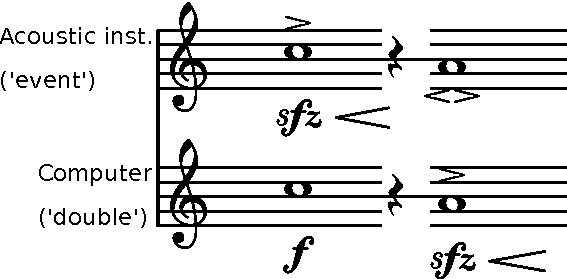
\includegraphics[width=.75\linewidth]{img/lily-interaction}
  \caption[Simplified example of real-time pitch and onset interaction.]{Simple example showing immediate real-time pitch and onset interaction with a second layer of deferred musical dynamic interaction.}
\label{fig:interactive-1A}
\end{wrapfigure}
In the (trivial) example in \hyperref[fig:interactive-1A]{Figure \ref*{fig:interactive-1A}}---a transcription of a fictitious instrument-computer improvisation---the computer `double' follows the pitch and the on/offset times of the `event' in one-to-one mapping. In this regard the response from the computer system corresponds to an immediate and unaltered mirror image. In a second interactive layer, however, the `double' appears to be using dynamic information, i.e. the amplitude envelope, of the note event prior to the current. On the second note in time the `double' mimics the \emph{\textbf{sforzando}}--\emph{\textbf{crescendo}} amplitude curve of the first note of the `event' voice. One may imagine more subtle effects such as introducing temporal tension between the two notes in the domain of timbre; micro-variations in tone colour whose greater shape is asymmetrical, that is unrelated, but whose coming into existence is interactive but deferred in time, etc. The point here is not \emph{what} is done but to show that different compositional strategies\footnote{Working out \emph{what} and \emph{how} in an interactive system in music is tantamount to traditional composition.} may be employed and that interaction may take place on multiple co-existing temporal levels, exploiting different levels of contraction. If, however, the one-to-one mapping of pitch and duration is blurred, if it is not absolutely clear that the `double' is following the `event', that distortion is likely also negatively to influence the deferred time interaction.\label{par:label:human-comp-inter:9} \hypertarget{par:human-comp-inter:9}{If the purpose} in this example (for the moment disregarding the amplitude envelope delay) is defined as \emph{the wish to extend electronically the sound of the acoustic instrument by means of superimposing an electronically generated timbre upon it}, proximity in time is of the essence. A lag or delay in the electronic voice in relation to the acoustic---a delay between `event' and `double'---will create a positively \emph{different} musical gesture compared with the intended effect. If the discrepancy between attack times is sufficiently large, the desired effect of extension of the acoustic sound will fail and the two sounds will instead be perceived as separate musical events. An inconsistent rhythmic displacement may create an interesting gesture but the result is still different from the intention to a considerable degree. The difference between the `double' in \index{real-time}\index{time!real-time}real-time and the `double' in independent time, however, does not merely make up two different tokens of the same type: they constitute two different types of paradigms, two different classes of systems. In essence it is the difference between the extension of an instrument and the extension of a \useGlosentry{glos:musician}{musician}.

%Hence,  Which is not to say that a delay between event and double, between stimulus and response, is not a time for interaction, exchange and negotation. (A time allowing for a different role of the listener?) 

% ``Everything is in motion, eveyrything is changing, everything is % being transformed and yet nothing changes. Such a society, thrown into % technological progress, accomplishes all possible revolutions but % these are revolutions upon itself.''(Baudrillard cited in plant, p. % 35)

\section{Interactive paradigms---\emph{interaction-as-difference}}
\label{sec:inter-parad}
%Context is paramount to the discussion of the significance of rhythmic synchronization. 

As I have attempted to show, \citeauthor{baudrillard02}'s statement that the more perfectly synchronised the `event' and the `double', the lesser the value of the exchange is contestable. Not because it is wrong (I believe it is right), but because, as so often happens, in practice theories rarely play out so symmetrically and because of the particularities of music and time. The importance of \emph{imprecision} \hyperlink{par:human-comp-inter:8-1}{has been discussed} but the aspect of precision may be, depending on the view, equally important. In essence it is a question of context and intention because rhythmic simultaneity and precision may be absolutely critical for some music and equally devastating for others. To explore these issues in the context of interactive computer music, let us consider the important aspect of the purpose as defined in the earlier example in Figure \ref{fig:interactive-1A}: \emph{to extend the sound of the acoustic instrument by superimposing an electronically generated timbre upon it}. This is the intention against which the result is to be measured. It is a simple case of an instrument-computer performance, with a hypothetical, overly simplified, instruction algorithm along the lines of:
%
\begin{equation}\label{eq:1}
  \emph{whatever pitch `heard' $\Rightarrow$ play the same}
\hypertarget{eq:human-comp-inter:1}{}
   \end{equation}
%
Now this could well be a postcard piece by James Tenney\footcites(The \citetitle{tenney04} is a series of eleven short and minimally stated compositions, ``scorecards'' printed on postcards, composed by \citeauthor{tenney04} in the early 1970s.)(){tenney04}[see~also][]{risset87} or an instruction for an improvisation. It is a compositional statement, albeit an open one, but when the rule of synchronicity is introduced as a factor there occurs a major change as far as the freedom and openness is concerned:
%
\begin{equation}\label{eq:2}
\emph{if played note occurs later than original $\Rightarrow$ error}
\hypertarget{eq:human-comp-inter:2}{}
\end{equation}
%
This may also be a viable function to attempt solving the result of which may well be interesting from a musical as well as a technological point of view. Together the two lines form a compositional statement that to a considerable degree limits the independence of the agent to whom these instructions are given. To define restrictions such as these, though it is a perfectly normal musical behaviour, is to issue a control agency. In the Western music tradition where concepts such as \emph{\index{Werktreue}Werktreue}\footcites(The German word \emph{\index{Werktreue}Werktreue} means `to be faithful to the original'. It is commonly used in discussions concerning musical interpretation and musical \index{ontology}ontology.)()[See][3]{benson03}[See also][]{goehr96} have played an important role, the idea that one \useGlosentry{glos:musician}{musician}---usually the composer or the conductor---controls or limits the freedom of another is perfectly normal, in particular from the perspective of those who exercise the `control'.\footnote{Similarly to how the aspect of real-time communication discussed by \citeauthor{baudrillard02}, although despised by him, is intended, desired and profited from by the control agency that governs it.} Furthermore, restricting and reducing the number of choices possible in a given context may promote rather than limit creativity.\footcite[See][chap. 4]{evens05} Regardless of these aspects, however, by adding time to the algorithm---though it is not time \emph{per se} but the values assigned to time in this example---the mode of interactivity is approaching the \hyperlink{sec:inter-defin:par4}{previously discussed} \index{interaction!as control}\index{interaction-as-control}interaction-as-control.

To  complicate this perhaps trivial example, the \emph{role} of the musical `double' in an \index{interaction!interactive music system}interactive music system such as the one described here should be considered. Where does its centre position lie on the `instrument'---`player' continuum?\footcite[For a description of the classification system from which this terminology is borrowed see \autoref{sec:music-pract-inter}. See also][]{rowe01} 
%Section
That is, to what extent is the `double' also able to contribute actively to the music as opposed to merely following instructions? By no means is this a simple distinction to make, nor are `player' and `instrument' separate and irreconcilable categories. Any instrument, \index{digital}digital or analogue, electronic or acoustic, will contribute to the music through its history, its physicality and its limitations as well as through many other parameters. The seemingly opposing paradigms of `player' and `instrument' are perhaps best described as related classes with many common members where the `player' class \emph{extends} the functionality of its parent `instrument' class (a `player' will need some kind of an `instrument' on which it  `plays'). Perhaps the process of categorising a system within these classes will have to be done pragmatically, not based on the properties of the computer and its \index{software}software, but rather on the \emph{usage} and \emph{purpose} of (using) it. If I have a distinct intention about \emph{when}, with \emph{what}, and \emph{how} I want my computer to respond (musically), then I am essentially designing an `instrument'. If, on the other hand, I am primarily interested in engaging in a mutual exchange with the computer, then I am essentially implementing a `player'. In this context the consequential difference between the two methods is that the latter has only a vaguely formulated, system-specific, rationale against which the output may be evaluated,\footnote{If the played note by a given `player', that implements the rule in \hyperlink{eq:human-comp-inter:1}{a quasi algorithm \eqref{eq:1}}, is not equal to the most recent note analysed, it only means the current played note is not the most \emph{recent} note analysed, which is not an error according to the rule. The most recent note analysed may appear at some later point in time.} one where there is room for interpretation and difference. The former, on the other hand, includes preconditions that make possible an unambiguous evaluation of the output in relation to the input (such as the \hyperlink{eq:human-comp-inter:2}{second rule above}).

The `instrument' paradigm, in the sense that it takes input from a source from which it generates an output based on a logical rule set, is a type of communication system. Information is sent from \useGlosentry{glos:musician}{musician} (sender) to `instrument' (receiver), and the sender expects to be in control of the system, i.e. expects that messages transmitted are received with a minimum of noise and that the system is able to decode the message correctly. In this description is also an expectation that the code does not change over time, a potential for developing a fluency on the instrument. \emph{\index{interaction!as control}\index{interaction-as-control}Interaction-as-control}. Within the `player' paradigm the streams of communication are not unidirectional. The code of the communication may in part be negotiated in the course of action. The value and meaning of noise are different. A `player' system approaches a circular cause-and-effect system, a container for feedback, a \index{cybernetics}cybernetic system. If what comes out of it is not satisfactory according to some standard---a standard imposed and set in runtime rather than, as is the case with an `instrument', pre-runtime---it is up to either part to alter its behaviour and attempt to create the desired change to approximate the criterion, to initiate a big enough difference to modify the balance and cause a system change. \emph{\index{interaction!as difference}\index{interaction-as-difference}Interaction-as-difference}. Despite the reductive way the two paradigms `instrument' and `player' were portrayed by the simplistic rules in the \hyperref[sec:inter-parad]{examples above}, I believe they bear evidence of the different kinds of interaction they encourage. It is equally true, and important to remember, however, that the same system may in fact display different characteristics depending on the posture of those who engage interactively with it. This is not the sole property of electro-acoustic instruments, but just as true for any musical instrument.

%Though it is possible here, as well as in the former system, to measure the information content in the communication, without the formal, predetermined rules, without the code, the simple logic (if $x$, then $y$)former system \emph{may} be used here but the data validation process is considerably more complex. 

%These systems are still abstract models. The point here is not to discuss the possible implementation, though it should be mentioned that the `player' system, fully expanded would constitute a very complex system. As models they portray differences where the most conspicuous is that status of noise and error. In the first noise should be avoided and errors are identifiable. In the second noise is par of the message and errors are generally indeterminable.

%The consequences of the latter is also that I must accept `faulty' or unexpected output from the computer, and `errors' or noise in my `signal' should preferably not cause a system havoc. 

In the discussion above I have attempted to reveal the compound nature of the matter of interaction and time. Within it are concealed issues relating to causality, embodiment, expression, social exchange, the Other, and many, many more. The question I have tried to address here is how and if the \index{real-time}\index{time!real-time}real-time interaction of communication is related to the \index{real-time}\index{time!real-time}real-time of \index{interaction!musical}musical interaction and an unwrapping of some of the different kinds of time at play. As was mentioned towards the end \hyperlink{par:human-comp-inter:10}{of Section \ref*{sec:time-interaction}}, \citeauthor{baudrillard96}'s point is that what he calls symbolic exchange, essentially \index{interaction!social}social interaction, depends on time; it feeds on the suspense that is the result of the delay between cause and effect, whereas the \index{real-time}\index{time!real-time}real-time of the \index{virtual}Virtual is the effectual abolition of both time and distance. For the moment disregarding the fact that a different analysis of communication and time in the sphere of the \index{virtual}Virtual is possible,\footcite[E.g.][chap. 11]{levy97} it is obvious that the relation between time and meaning is of a different kind when the realm of musical performance is entered. The thought that expression and `meaning' would increase with \emph{\useGlosentry{glos:latency}{latency}} in a musical instrument is preposterous. (It would make the church organ the most expressive instrument and something like the violin the least expressive.) Further, the time and rhythm of \index{interaction!social}social interaction are even more pertinent and present in music and I have argued that, even if the interaction (in music) is limited to a simple trigger-response metaphor of communication, time is still at play, by the very nature of music. For a traditional musical instrument the interaction between it and the musician is governed by the \index{real-time}\index{time!real-time}real-time information (feed-back) but \emph{also} by the musician's embodied knowledge about playing that particular instrument design, and by the intellectual memories of playing and learning how to play (and a myriad of other memories). Therefore, even if it seems like the playing is taking place in \index{real-time}\index{time!real-time}real-time, many other kinds of time and interactions are taking place on lower levels. Some of this knowledge is more or less consciously encoded into memory and some of it is entirely beyond control and influence.
%, such as deterioration of the instrument, physical proerties of the room we are in, psychological changes, etc.


%In practical terms: I don't have to re-learn how to play the saxophone when I pick up a new instrument, one I have never played before, because the interactive knowledge is not tied to the specific object but to the general concept of the instrument.



%The perhaps most pressing question is what the relation is between human-computer interaction outside of the field of musical practice and musican-computer interaction inside that field. 

\section{Multiplicities of musical interaction }
\label{sec:mult-music-inter}


\hypertarget{sec:human-comp-inter:par8}{The development} that led to the \index{real-time}\index{time!real-time}real-time responsive computers discussed \hyperref[sec:interaction-time]{above} unquestionably gave birth to the possibility of a different mode of interaction, and the distinction between the prior, non-real-time interaction and the current \index{real-time}\index{time!real-time}real-time is relatively obvious. Reading \citeauthor{baudrillard96}'s \citetitle{baudrillard96:writing}, however, one may get the impression that \index{real-time}\index{time!real-time}`real-time' is a unanimous and clear-cut category of interaction. Between \index{real-time}\index{time!real-time}real-time and detained time, between high-definition and low-definition time, however, exist many layers of interactions that operate on different timescales, particularly in music. Ingrid \citeauthor{monson96}'s book \citetitle{monson96} takes this multi-layered nature of \index{interaction!musical}musical interaction (of jazz and improvised music) as its starting-point: ``Stressed here are the reciprocal and multi-layered relationships among sound, social settings, and cultural politics that affect the meaning of jazz improvisation in twentieth-century American cultural life''.\footcite[2]{monson96} Sounds do not interact in a void but depend on and become influenced by social and culturo-political interactions. She also makes use of the linguistic model of \index{interactional texts}\index{Monson, Ingrid!interactional texts}\index{interaction!interactional texts}`interactional texts', briefly 
\hyperlink{sec:inter-defin:monson}{discussed above}, which allows us to identify the multiplicity and simultaneity of musical communication, as many of these `texts' may operate concurrently. \citeauthor{monson96} writes that ``the intersection of all of these roles [\ldots] contributes to the way in which interactionally produced musical texts develop'' and that ``these interactionally produced events structure both musical and social space''.\footcite[189-90]{monson96} \citeauthor{monson96} assembles different modes of interactivity and shows that these are all part of, and present in, the musical performance. The minute adjustments made within the jazz rhythm section to accommodate the groove may at the same time seem enigmatically indulgent\footcite[For a study on the rhythmic variation present in jazz, see][]{friberg02} and incredibly sensitive to variation. On one level, the interaction within the rhythm section certainly takes place in very high definition and it must be said to conform with what \citeauthor{baudrillard02} calls the inexpiable `live' time. Along with this \index{real-time}\index{time!real-time}real-time interaction, however, are many other levels of interdependent interactions such as those formed by interpersonal relations, as mentioned by \citeauthor{monson96}. These manoeuvre in a different time but may well influence, and depend on, the lower level \index{real-time}\index{time!real-time}real-time interactions.

Is this not true also for \index{interaction!human-computer}\index{HCI}human-computer interaction? That the social and political interactions that relate to the different aspects of technology inform not only the technology itself but also how one interacts with it? Or is the nature of the `virtual', digitally encoded as it currently is, so radically different from the social dimension---the `world' as \citeauthor{baudrillard02} would refer to it---that, in the encounter, any formerly constructed interactive texts are inescapably eradicated and all that remains is the  \index{real-time}\index{time!real-time}real-time \index{virtual}virtual representation? The deceptive distinction between \index{real-time}\index{time!real-time}real-time and non-\index{real-time}\index{time!real-time}real-time mentioned above is mirrored in an equally deceptive distinction between real and \index{virtual}virtual. Now this is irrefutably one of \citeauthor{baudrillard02}'s main points,\footnote{Hyperreality is the process of making the representation of the world more real than the real world, hence making it difficult to distinguish the real from the virtual.} but for him, although one may be mistaken for the other, the real and the \index{virtual}virtual are mutually exclusive: ``for it is the particularity of the \index{virtual}virtual that it puts an end not just to reality, but to the imagining of the real, the political and the social; not just to the reality of time, but to the imagining of the past and the future''.\footcite[107]{baudrillard02} As the extension of \index{hyperreality}hyperreality the \index{virtual}virtual scrambles and destabilises truth and the real. Eventually the \index{virtual}virtual claims the real, for there ``is no room for both the world and its double''.\footcite[34]{baudrillard96} As was mentioned earlier in relation to the Situationist's notion of the \index{Spectacle, Society of the}\index{Debord, Guy!Spectacle}Spectacle, \citeauthor{baudrillard96} states that there is no escape from the \index{virtual}virtual because it keeps no trace of the real, of the earlier world. This, he says, makes it a hypothesis with much more far-reaching consequences than \citeauthor{heidegger93}'s notion of \emph{\index{Heidegger, Martin!enframing}enframing} because, just as there is a possibility for reversal in Debord's description of the \index{Spectacle, Society of the}\index{Debord, Guy!Spectacle}Spectacle, \index{Heidegger, Martin!enframing}enframing is both ``\emph{danger} in the highest sense''\footcite[333]{heidegger93} and holds within it the potential for ``the rising of the saving power''.\footcite[338]{heidegger93}

\section{Interaction and the Digital}
\label{sec:interaction-digital}


\hypertarget{interaction-digital}{The cross-disciplinary scholar Aden \citeauthor{evens05}}, in a chapter of his book \citetitle{evens05} entitled ``The  Question Concerning the Digital'', approaches \citeauthor{heidegger93}'s ponderings on technology, but, as can be told from the title, centres on the \emph{digital} as a defining property of modern technology, as its uniting power. Because the \index{digital}digital is the code which allows for the representation to be infinitely reproduced, because it introduces order, consistency and generality into the world, \citeauthor{evens05} identifies the \index{digital}digital as a result of the technology's \index{Heidegger, Martin!enframing}enframing\footnote{The German word used by \citeauthor{heidegger93} is \emph{Gestell}, which is commonly translated as \emph{enframing}. Aden Evens, however, suggests the English translation should be \emph{set upon}, which is what he uses consistently. \cite[See][182n2]{evens05}. In the translation of \citetitle{heidegger93} that I am using, however, a distinction is made between \emph{setting upon} and \emph{enframing}.} of nature. Truly, the binary system is an excellent example of generality, the ultimate abstract code which chops up nature in infinitesimal slices (frames?), each of which is further sliced up and every `bit' is assigned a zero or a one. The represented object is not just reproducible, it is comparable (a binary distinction for each bit) and communicable (a stream of numbers is easy to transmit). It is \index{digital}digital. \citeauthor{evens05} distinguishes the \index{digital}digital as ``purely formal'' and as such it ``grasps only form and so falls ever short of actuality''.\footcite[66]{evens05}  As was \hyperlink{sec:human-comp-inter:par5}{mentioned earlier}, according to \citeauthor{baudrillard02} the commodity has gone through a process of complete and total abstraction, an annihilation of meaning, whereafter it signifies only itself. \citeauthor{evens05} makes the connection\footnote{Aden \citeauthor{evens05} refers to \citeauthor{baudrillard02}'s \index{digital}digital interpretation of the Twin Towers in New York City.} and points to the singular nature of the \index{digital}digital and its inability ever to point beyond the plane of the \index{digital}digital: ``It represents but does not present''.\footcite[76]{evens05} In his text the \index{digital}digital is given a thorough and very readable investigation, expanding the concept well beyond a mere binary system of digits. \citeauthor{baudrillard96}'s \index{virtual}virtual/real dichotomy, mirrored in \citeauthor{evens05}'s \index{digital}digital/actual, is because of the multiple perspectives provided by \citeauthor{evens05} (represent/present, general/singular) considerably blurred. But the more important distinction here is that, whereas \citeauthor{baudrillard96} finds the \index{virtual}virtual transformation immutable, although \citeauthor{evens05} identifies serious limitations of the \index{virtual}`virtual' (limitations he traces back to the formality of the \index{digital}digital), he also sees the possibility for it to transcend its own medium and become a dynamic and ``organic aggregate''.\footcite[78]{evens05} When \citeauthor{baudrillard02} sees the `sampling' of our world as irrevocable and a sign of the complete failure of Heidegger's quest to hold the dangers of technology before our eyes, \citeauthor{evens05} traces Heidegger's notion of the \emph{saving power} of technology to the \emph{interface} between \index{digital}digital and actual. Further obscuring the \index{digital}digital/actual boundary, \citeauthor{evens05} states that: ``the digital is not on its own, as it engages constantly with the human world of actuality''. It engages with the world, through humans, mediated by the interface between the \index{digital}digital and the actual. Perhaps one could say that in this process, the \index{digital}digital representation of the world is `de-framed'. \citeauthor{evens05} argues that ``whatever vitality, whatever creativity inheres in digital technologies, [\ldots] will be found in [the] interstitial zone''; the fuzzy boundary of the \index{digital}digital.\footcite[79]{evens05}

\label{sec:interaction-digital-1}
The interface, as discussed \hyperref[sec:human-comp-inter]{above}, allows access to technology and the activities involved constitute the human-technology interaction. According to \citeauthor{evens05} the space between the \index{digital}digital and the actual, the ``ambiguous space of transformation'',\footcite[80]{evens05} is a space occupied by the interface, or by the technologies that make up the interface (the mouse, the keyboard, the icons on the screen, etc.). So the (\index{digital}digital) content is challenged by the user through the interface. But where do the data end and the interface begin? (The conflation between text and link in hypertext is an example of the difficulty in delimiting data from interface: the text is both content \emph{and} interface.) And by what standard is the (\index{digital}digital) computer interface \emph{less} \index{digital}digital than the data it makes available? If it too is purely \index{digital}digital, in what way does it open a channel to the data that makes it more accessible to the sphere of the actual, more alive? \citeauthor{evens05} maintains that, because the interface mediates between the user and the computer, it is by definition a hybrid of both \index{digital}digital and actual, but the hybrid is accomplished, not by making the (already \index{digital}digital) interface more actual, but by the user submitting to the formal reduction of the \index{digital}digital.\footcite[80]{evens05} In order to move across the actual/\index{digital}digital boundary one has to succumb to the \index{digital}digital and herein lies the danger, the threat, of the \index{digital}digital: ``by requiring each user to conform to its standards, it imposes a uniform experience that not only reduces the world to a pure formality but offers to each of us the same formalities, the same possibilities, the same pseudo-creativity''.\footcite[81]{evens05} This twofold nature of the \index{digital}digital as both potential and threat is a reflection of \citeauthor{heidegger93}'s ruminations on the \emph{dangers} and the \emph{saving powers} of technology. By reference to German poet Friedrich H\"{o}lderlin, \citeauthor{heidegger93} claims that the two aspects are never mutually exclusive but always potentially co-existent.\footcite[The lines by H\"{o}lderlin are: ``But where danger is, grows / The saving power also''. Quoted in][333]{heidegger93}

\label{sec:interaction-digital-2}
Therefore, the interface allows for interaction, and following \citeauthor{evens05}, it binds together the user and the computer; a glue without which the \index{digital}digital would remain inaccessible. Metaphorically speaking, the interface \emph{creates} interaction. This model gives the impression that the user \emph{is} the actual and the computer \emph{is} the \index{digital}digital and that these two agents are utterly incompatible unless one approaches the other. Because the \index{digital}digital is static and unchangeable, trapped in its own formality, of the two only the user, i.e. the human, is capable of altering him/herself to approach the \index{digital}digital through the interface. As a consequence, has the user ceased to be \emph{only} actual? \hyperlink{sec:inter-defin:par4}{Going back} to the concept of \index{interaction!as control}\index{interaction-as-control}interaction-as-control, common to much of \index{interaction!human-computer}\index{HCI}human-computer interaction, given the \index{digital}digital/actual dichotomy so thoroughly explored by \citeauthor{evens05}, in order for the user to exercise control over the computer s/he has to become the computer to a certain extent, give something up, give in to gain. (To gain, because, after all, something is returned or computers would not sustain such interest.) This duality is identified by McLuhan when he states that ``any technology is an extension or self-amputation or our physical bodies'',\footcite[49]{mcluhan01} paraphrased and extended by \citeauthor{baudrillard02} to the somewhat more radical and acrimonious ``[technology is the] expulsion of man''.\footcite[35]{baudrillard96} Is the reconfiguration demanded by the user, as the prerequisite for \index{interaction!human-computer}\index{HCI}human-computer interaction, a staging of this extension/amputation/expulsion? Is the giving up of a part of our selves in order to embrace technology\footcite[McLuhan writes that to ``behold, use or perceive any extension of ourselves in technological form is necessarily to embrace it''.][49]{mcluhan01} really specific to interaction with technology? Is the request of the \index{digital}digital that we give in, just a little bit, to its mode of operation not a natural component of any kind of interaction? I \emph{approach} the other in the interactive invite by `reconfiguring' my senses to her, albeit slightly, give up a part of my \index{Self}self and, in the process, I also extend myself.

\label{sec:interaction-digital-3}
Towards the end of ``The Question Concerning the Digital'' the very interesting idea of ``a dialectic of interface and data [that] also implicates the user''\footcite[80]{evens05} is introduced. As the interface is refined, argues \citeauthor{evens05}, the \index{digital}digital data are forced to reorganise and the users, for their part, keep pressure on the interface and the \index{digital}digital, which, in this operation, is pushed to become more than it is,  challenged, and ``the pipe that passes from the \index{digital}digital to the actual bursts its seams to carry the \index{digital}digital beyond itself''.\footcite[81]{evens05} These thoughts open up an alternative, less machine-centric view on how to think about and attempt to understand technology/virtual/\index{digital}digital. I argue that in the dialectic of interface, data and user the interaction is the central aspect. The interaction \emph{creates} the interface. A `good' interface is one that allows itself to be created.\footnote{The most obvious and tangible example within the realm of computer music is the \index{Pure Data (PD)}\index{Puckette, Miller}Pure Data (PD) by Miller Puckette. Its interface is recreated for every instance, every project, every interaction, every iteration. \cites[See][]{puckette96}[and][]{puckette07}.} In this model the user does not constitute the actual, s/he is primarily \emph{part of} it and similarly the computer is primarily \emph{part of} the \index{digital}digital. Actual and \index{digital}Digital are two types, two classes that can have any number of members and whose structure is somewhat amorphous. The more the agents of different classes interact with each other, the more the two classes overlap and the more they inherit properties from each other and the larger, less rigid and more fluent becomes the interface: the union between the two classes. The more `information' one class has about the other, the more likely is the interactive field to grow. The more rivalry there is the more likely it is to vanish. Knowledge about the Other is the key to avoiding fear and conflict.

\label{sec:interaction-digital-4}
In this section the Real/\index{virtual}Virtual opposition favoured by \citeauthor{baudrillard02} has been compared with Aden Evens's Actual/\index{digital}Digital distinction, a dichotomy that consists of categories that may be slightly misleading and not as clear cut as they appear. The \index{digital}Digital is used by Evens in an attempt to avoid the technology and instead focus on the structure of technology. This is comparable to how Heidegger points to the \emph{essence} of technology rather than technology itself which, in both cases, allows for philosophical rather than a technical discussion. The `Actual' as category is the negation of the \index{digital}`Digital' and silently points to Heidegger's `truth' or `nature'. But is the \index{digital}digital encoding a property of technology only? What is a fired neuron in the brain if not a binary transition? In a discussion on cybernetics Gregory Bateson writes that ``in the vast majority of instances, the neuron either fires or does not fire'' and he goes on to explain how ``it is possible to make systems out of \index{digital}digital neurons that will have the \emph{appearance} of being analogic systems''.\footcite[103]{Bateson} In other words, according to \citeauthor{Bateson}, the human brain has certain low-level qualities that may be seen to lean towards the \index{digital}digital. Similarly, through the use of artificial neural networks, it is possible to simulate an analogue system by \index{digital}digital means. This affinity between categories makes it possible to look at \index{interaction!human-computer}\index{HCI}human-computer interaction in a way less focused on opposition and resistance and more on exchange. Described as classes, the \index{digital}digital and the actual can reciprocally exchange properties or modes, without losing their mutual identity. Furthermore, instances of these classes---the agents of the interaction---construct the interface through which data may pass and in these inter-agent transactions the participants have to acknowledge each other.

%Although the `Real' must be understood in relation to a philsophical context as `truth' or `nature' and thereby outside the scope of this discussion, the `Virtual' as a place where technology interaction takes place is problematic. In what constist the difference between a dream and 

\section{Interaction and symbiosis: Cybernetics}
\label{sec:interaction-symbiosis}

%The important aspect of time and interaction, also discussed \hyperref[sec:interaction-time]{in section \ref*{sec:interaction-time}} is 

%Apart from the discussion on \ref{sec:inter-defin:par4}musical interaction and the briefly mentioned debate on intelligent agents

Before the \index{digital}digital revolution, and some twenty years before the \index{PC}\index{Personal Computer}PC, Joseph Licklider---whose significant work was briefly mentioned \hyperref[sec:human-comp-inter]{above}---imagined the future of \index{interaction!human-computer}\index{HCI}human-computer interaction and computation as one devoid of ``inflexible dependence on predetermined programs'' where computers and humans would develop a symbiotic relation. In \citeauthor{licklider60}'s vision the computer usage paradigm would shift from the user supplying the computer with a pre-formulated problem to one in which the user and the computer ``cooperate in making decisions and controlling complex situations''.\footcite{licklider60} Although \citeauthor{heidegger93}, \citeauthor{baudrillard02} and \citeauthor{evens05} have focused on the problems of the dissimilarities and incompatibilities between technology and its users they have all to various degrees considered the dangers and the subsequent destructive aspects of technology and pondered on ways in which it may be altered, to become more human, \citeauthor{licklider60}, while identifying the same dissimilarities, saw great potential in them. To \citeauthor{licklider60}, the human-computer incongeniality was a possibility rather than an obstacle, a possibility for computers to complement humans in difficult and perhaps mundane tasks. His categorization of the two parts of a human-computer system is a rough summary of the challenges involved in human \index{interaction!computer}computer interaction:

\begin{squote}
As has been said in various ways, men are noisy, narrow-band   devices, but their nervous systems have very many parallel and   simultaneously active channels. Relative to men, computing machines   are very fast and very accurate, but they are constrained to perform   only one or a few elementary operations at a time. Men are flexible,   capable of ``programming themselves contingently'' on the basis of   newly received information. Computing machines are single-minded,   constrained by their ``pre-programming''. Men naturally speak   redundant languages organised around unitary objects and coherent   actions and employing 20 to 60 elementary symbols. Computers   ``naturally'' speak non-redundant languages, usually with only two   elementary symbols and no inherent appreciation either of unitary   objects or of coherent actions.

To be rigorously correct, those characterizations would have to   include many qualifiers. Nevertheless, the picture of dissimilarity   (and therefore potential supplementation) that they present is   essentially valid. Computing machines can do readily, well, and   rapidly many things that are difficult or impossible for man, and   men can do readily and well, though not rapidly, many things that   are difficult or impossible for computers. That suggests that a   symbiotic cooperation, if successful in integrating the positive   characteristics of men and computers, would be of great value. The   differences in speed and in language, of course, pose difficulties   that must be overcome.\footcite[Section 3.1]{licklider60}
\end{squote}

The language problem---which in this context is an issue of information encoding and hence related to the \hyperlink{interaction-digital}{discussion of the \index{digital}digital}---cannot be said to have been overcome. Computers still do not generally ``speak'' redundant languages and even if higher-level computer languages have been developed, these are far from spoken inter-human communication. Further, if the computer according to \citeauthor{licklider60} was too fast in 1960 (for the purpose of symbiosis), considering that the input devices are roughly the same whereas the computer speed capacity according to Moore's law has doubled 32 times since then,\footnote{Gordon Moore predicted in 1965 that the number of transistors on a computer chip, and hence the processing power, would double every 18 months ($1960\Rightarrow2008=48$ years, $\frac{48\times12}{18}=32$). To be fair, Moore's law was not formulated until 1965 and in reality it seems as if the doubling has actually happened on average every 20 to 24 months. All the same, computers have grown much faster and the means for interaction has not changed in any radical way.} speed according to the same standard must still be an issue. Despite these issues concerning speed and language, however, are we not already living the \index{symbiosis, man-computer}man-computer symbiosis predicted by \citeauthor{licklider60}?

On the one hand it is fair to say that we are. We are living interdependently and in close union with computers in what could be called a symbiotic relationship. (After all is not the greatest fear, the most commonly explored horror of science fiction, that one day computers may not need us?) To deal with the speed issue, \citeauthor{licklider60} envisioned resource distribution by means of time-sharing that implemented `thinking centres', the equivalent of ``present-day libraries'', where one machine can serve multiple users (in essence a client/server protocol). With striking accuracy he draws the outlines of that which is to become the Internet: ``The picture readily enlarges itself into a network of such centers, connected to one another by wide-band communication lines and to individual users by leased-wire services''.\footcite[Section 5.1]{licklider60} The Internet as a thinking centre in a symbiotic relation with humans. In a search of the Internet not only answers are produced; just as many new problems are formulated. Though in reality it is arguable whether the Internet and the typical use of the Internet would qualify as one part in a symbiotic relation, the Internet in the sense of information collection was one of the aspects \citeauthor{licklider60} envisioned as part of \index{symbiosis, man-computer}man-computer symbiosis.

On the other hand, judging from Steve Dietz's paper \citetitle{dietz02}, in which the first dream is \citeauthor{licklider60}'s dream of \index{symbiosis, man-computer}man-computer symbiosis, we are still far from that vision. As one of the curators\footnote{Another curator was Electronic Music Foundation founder and president Joel Chadabe.} for the \emph{2003 New York Digital Salon}\footcite{digitalsalon03} \citeauthor{dietz02} examines ten dreams of technology that are not yet `true' or `real' (outside the realm of art, one may add), but which all have a future, ``even if we do not yet know what it is and despite the certainty with which it is predicted''.\footcite{dietz02} \hypertarget{sec:target:interaction-symbiosis}{Though many artists} have dreamed the dream of symbiosis, the artwork \citeauthor{dietz02} associates with man-machine symbiosis is David \citeauthor{rokeby91}'s installation \citetitle{rokeby91}. As an interactive installation\footcite[For an introduction and description of the work, see][]{rokeby91} it engages with the visitor in a sophisticated feedback process. The visitor places objects, toys and household objects that the computer `sees', analyses and assign names to. Over time it builds relations between the objects and, through the use of speech synthesis, it starts building phrases out of its repository of the object/name couples that it reads back to the visitors.

In \citetitle{rokeby91}, the visitor and the computer interact through (are mediated by?) the objects and through the voice of the speech synthesis engine. By placing objects in the computer's line of sight the visitor teaches it something about the world and through the computer's accumulated knowledge, the visitor is told something about the world from a slightly skewed perspective. As regards the topic of interaction, though there are many interesting aspects of \citetitle{rokeby91} that intersect with the discussions in the current text, the \hyperref[sec:interaction-time]{question of time} (see also the discussion relating to \hyperlink{sec:human-comp-inter:7}{\index{real-time}\index{time!real-time}real-time \index{interaction!musical}musical interaction}) is particularly well illustrated. \citeauthor{baudrillard02}, who obviously felt strongly about this, pointed to the \index{real-time}\index{time!real-time}real-time aspect of the \index{virtual}virtual as inexpiable: ``it is the particularity of the \index{virtual}virtual that it puts an end not [\ldots] just to reality of time, but to the imagining of the past and the future''.\footcite[107]{baudrillard02} It is the immediate return, the expeditious reply, that kills the past and the future and turns everything into a singular moment. Whether one agrees with \citeauthor{baudrillard02} or not, the concept of \index{real-time}\index{time!real-time}real-time must be expanded beyond its use in \index{interaction!human-computer}\index{HCI}human-computer interaction because, as was seen towards the \hyperlink{par:human-comp-inter:8}{end of Section \ref*{sec:time-interaction}}, \index{real-time}\index{time!real-time}real-time interaction, the instantaneous proximity of events, has crucial significance in \index{interaction!musical}musical interaction. Within the realm of computers there are several different types of \index{real-time}\index{time!real-time}real-time; there is the \index{real-time}\index{time!real-time}real-time interaction as well as the related but yet different aspect of \index{real-time}\index{time!real-time}real-time computation. \index{real-time}\index{time!real-time}Real-time interaction depends on \index{real-time}\index{time!real-time}real-time computation but the latter does not necessarily have to implement the former. 

As a system, \citetitle{rokeby91} relies on a number of different interactive modes of which \index{real-time}\index{time!real-time}real-time computation is one of the important ones. Without it, the project would not have been possible: The computer would not have been able to process the images from the camera (constituting its `line of sight'), nor would it have been able to `read' the texts back to the visitors. Yet the communication between the visitor and the \index{virtual}virtual world of the installation does not take place in the kind of one-dimensional click-and-response \index{real-time}\index{time!real-time}real-time that \citeauthor{baudrillard02} objects to. Rather, because of the way the \index{software}software accumulates `knowledge' about objects displayed to it over time, the communication is based on present \emph{and} past experiences, not just the current. Therefor, the interaction only becomes meaningful if both parties accept that they engage in the exchange coming from different backgrounds and that mutual respect for this past is shown. \hyperlink{sec:inter-defin:par4}{\index{interaction!as control}\index{interaction-as-control}Interaction-as-control} is not possible, not meaningful, because the main interactive mode is based on exchange, feedback and reciprocity on a number of simultaneous layers of time. As \citeauthor{dietz02} writes: ``The symbiotic feedback loop infers that over the course of more than a decade, the computer `learns' more and more about the world, and its oblique, almost Delphic utterances of our mundane combinations of boot and rubber-duck-and-ball objects also causes us to perceive the world differently''.\footcite{dietz02}

\citetitle{rokeby91} and the idea of man-machine symbiosis are in essence \index{cybernetics}cybernetic ideas. As a discipline and a meta-theory cybernetics is concerned with (among other things) ``control and communications in the animal and machine'',\footcite[There are many definitions of cybernetics---this one is from Norbert Wiener's \emph{Cybernetics} (1960), as cited in][]{cybernetic08} by themselves and together. \citeauthor{licklider60} defined one of the main aims of \index{symbiosis, man-computer}man-computer symbiosis as the wish to go from systems that solved pre-formulated problems to systems that, in a symbiotic relation with a user, would (also) act by themselves and contribute to the formulation of the problem.\footcite{licklider60} If we define these as belonging to two categories of systems (non-symbiotic and symbiotic), one of the differences between them may be described in terms of energy. The non-symbiotic system accepts input given to it and responds according to some (pre-defined) logic. It is a causal system in which the energy is provided by the user. The user energises the system by posing the question, much like when a billiard ball strikes another and the motion energy is transferred from the former to the latter.\footcite[405]{bateson72:cyber} In the symbiotic system, on the other hand, ``the energy of the response is usually provided by the respondent. [\ldots] when a neuron fires another, or an impulse from a microphone activates a circuit, the sequent event has its own energy sources''.\footcite[409]{bateson72:cyber} Gregory \citeauthor{bateson72:steps} distinguishes this last category as a \index{cybernetics}cybernetic system, a communicational system with sequences resembling stimulus-response rather than cause-and-effect.\footcite[409]{bateson72:cyber} Feedback rather than click-and-response. Reciprocity rather than immediate reaction.

Again, it should be pointed out that in practice the difference between these types of systems is far from unequivocal, but, though there is nothing to say that a cause-and-effect system cannot incorporate some idea of time and memory, i.e. the system type itself does not exclude time, a \index{cybernetics}cybernetic system depends on it. Even the simplest \index{cybernetics}cybernetic unit displays ``a sort of determinative \emph{memory}'', because the ``stability of the system (i.e. whether it will act self-correctively or go into runaway) depends upon transformations of difference''.\footcite[317]{bateson72:cyber-self} Every part of the system will respond to changes and bits of information are passed around. Every such bit is ``definable as a difference which makes a difference'' and such differences are successively transformed through the internally interactive system.\footcite[315]{bateson72:cyber-self} In other words, the \index{cybernetics}cybernetic system needs to know, to remember, its state prior to current time and, preferably, have some notion of what the state of the other parts of the system is: it interacts internally with itself and with its environment. According to \citeauthor{bateson72:cyber-self}, these properties are what gives a \index{cybernetics}cybernetic system its holistic and mental features and his conclusion, of great interest from the point of the current project, is summarised in the following statement: ``[I]n no system which shows mental characteristics can any part have unilateral control over the whole. In other words, \emph{the mental characteristics of the system are immanent, not in some part, but in the system as a whole}''.\footcite[p. 316 (Italics by the author.)]{bateson72:cyber-self} Hence, in an interactive system in music that deploys some notion of cybernetics, the computer must not be seen as an isolated `player' but as part of a whole that includes the performer(s) with whom the system is interacting. Furthermore it will not be possible for the performer to gain control over the computer, or the computer over the performer, without the system failing or regressing. \index{interaction!as control}\index{interaction-as-control}Interaction-as-control relinquished in favour of \index{interaction!as difference}\index{interaction-as-difference}interaction-as-difference.

\section{Time and interaction revisited}
\label{sec:time-inter-revis}

\hypertarget{sec:target:time-inter-revis}{That} \citeauthor{baudrillard02}'s critique of \index{real-time}\index{time!real-time}real-time, however easily accepted, is not a property specific to the \index{virtual}Virtual \hyperlink{par:human-comp-inter:10}{has already been argued}, and I believe the brief analysis of \citeauthor{rokeby91}'s installation further corroborates it. More than anything the \index{real-time}\index{time!real-time}real-time of \citeauthor{baudrillard02} is a property and result of a general view of interaction, deflated and overly simplified by the all too common  and absurd notion of consumerism that `one-click-shopping' has given rise to. As a European inheritor of the visions of Joseph \citeauthor{licklider60}, Douglas Engelbart \footnote{D. Engelbart is commonly recognised as the inventor of the computer mouse, hypertext and ARPANET, the precursor of the Internet. Like \citeauthor{licklider60} in the early 1960s he argued for the use of computers to augment the human intellect. \parencites()()[See][viii]{levy97}[See also][]{johnson97}} and Marshall McLuhan,\footcite[See the foreword to][by R. Bononno]{levy97} French sociologist Pierre \citeauthor{levy97} whose visionary ideas on collective interaction were mentioned at \hyperlink{sec:target:inter-defin:par6}{the end of Section \ref*{sec:inter-defin}}, voices related criticism of the ``staccato, accelerated, quasi-punctual temporality of `interactivity'''.\footcite[125]{levy97} His book \citetitle{levy97} is concerned with opportunities and perils in network communities and nomadism made possible by the information highway. He supports the idea of multiple time configurations as well as the necessity of separating \index{real-time}\index{time!real-time}real-time, i.e. the sensation of time that emanates from interacting with \index{real-time}\index{time!real-time}real-time technologies, from the ``time experienced by the imagining community'' which will always overflow the the ``inadequacy of the immediate, of amnesiac channel hopping''.\footcite[125]{levy97} In other words, attempting to separate technology from the expression of technology.

I have now remarked several times on how interaction takes place in a \hyperlink{sec:human-comp-inter:par8}{multi-layered fashion} rather than in a singular type of interactional time, as is exemplified in some cases of \index{interaction!computer}computer interaction as well as \index{interaction!musical}musical interaction, and I have also suggested that the focal point of \citeauthor{baudrillard02}'s critique of the \index{real-time}\index{time!real-time}real-time interaction the \index{virtual}Virtual lies outside of the \index{interaction!human-computer}\index{HCI}human-computer interaction axis---and briefly hinted at \citeauthor{levy97}'s apparent support of this notion---but I return to the subject once again, for I believe it is one of the most important, and one of the most complex, aspects of music, let alone interactive music. Although Pierre \citeauthor{levy97} offers no consolation with regard to an actual, practical solution---I doubt that it is possible to find a solution that has relevance outside the realm of a specific context---he does provide a description of both the vision and the challenges of an understanding of time in a computer-mediated collective community:

\begin{squote}
The inadequacy of the immediate, of amnesiac channel hopping, no longer leads to lengthy sequences of interpretation, the infinite patience of tradition, which encompasses in a single sweep the ages of the living and the dead, and employs the quick currents of the present to erect a wall against time. [\ldots]

The rhythm of the imagining community resembles a very slow dance, a slow-motion choreography, in which gestures are slowly adjusted and respond with infinite precaution, in which the dancers gradually discover the secret \emph{tempi} that will enable them to shift in and out of phase. Each learns from the others how to make their entrance in stately, slow, and complicated synchrony. Time in the intelligent community spreads itself out, blends with itself, and calmly gathers itself together like the constantly renewed outline of the delta of a great river. The imagining collective comes into being so that it may take the time to invent the ceremony by which it is introduced, which is at the same time a celebration of origin and origin itself, still undetermined.\footcite[125]{levy97}
\end{squote}

The metaphor of the delta ties well with the \hyperlink{par:human-comp-inter:11}{Deluze/Bergson concept} of different degrees of contraction and relaxation. At the top of the delta, the present, the most contracted is encountered. It is also here that time flows by the most quickly after which a gradual slowing down begins until motion is no longer appreciable. The motion of slowing down is paralleled by the continuous relaxation in space as new branches of the delta are continuously unfolding, but the most striking aspect of this short excerpt is how \citeauthor{levy97} constantly refers to time as something which is created \emph{in between} participants, as something which spreads out. To him, there is no universal and superior time, but many ``\emph{tempi}'' (in plural) that comes and goes, some secret and shrouded in obscurity. 

% Are these the temporal variations that the `perfect' sequencer which typically has a `master clock' against which it synchronises its events (see the discussion in Section \ref{sec:time-interaction})


\section{Summary}
\label{sec:summary-1}

In this chapter I have discussed the topic of Interaction with regard to technology, and Interactive Music from a wide range of different angles. Interactive Music as a genre and as a practice has been probed and the wish to control computers in music has been questioned. The different meanings of interactive, interaction with regard to technology and \index{interaction!social}social interaction appear to be very different and it is suggested that there are many more kinds of interactions possible in the space between these outer posts. Heidegger's concept of the \index{Heidegger, Martin!enframing}enframing powers of technology is briefly touched upon. The recurring wish to use art to inform the field of \index{interaction!human-computer}\index{HCI}human-computer interaction is questioned and the difficulties, perhaps incompatibilities, between different fields of practice identified. Approaching the topic of time, and \index{real-time}\index{time!real-time}real-time, in the history of computation we see the significance and meaning of \emph{interactive} is revealed: real-time interaction because it is possible. The emergence of the interface as a mediator for interaction is discussed and a critique of the \index{virtual}virtual, a critique rooted in consumerism, is presented. In the critical attitude of \citeauthor{baudrillard96:writing} are also traces of possibilities for rethinking not only \index{interaction!human-computer}\index{HCI}human-computer interaction and the \index{real-time}\index{time!real-time}real-time but the critique itself. With the event--double terminology introduced in Section \ref{sec:time-interaction}, a few simple possibilities for different modes of interaction is presented. Then, in a departure from Robert \citeauthor{rowe01}'s interactive paradigms, the player and instrument models are presented in the context of a trivial example and the concepts of \index{interaction!as control}\index{interaction-as-control}interaction-as-control and \index{interaction!as difference}\index{interaction-as-difference}interaction-as-difference are introduced. Aden Evens's paraphrase of Heidegger is then approached and the \index{digital}digital characteristic is questioned as the possibility for a smooth transition from continuous to discontinuous is identified. Finally, the idea of man-machine symbiosis is revisited and it is suggested that a parallelism between man and computer should be allowed to replace the commoner trigger-response method.


% Interactive Music as a genre and the increasing impact computers are % having on our daily life. Adorno and Horkheimers concept of the % ``rationale of domination'' is brought up only to raise the question % of the role music may play with regard to the dominating powers of % technology. The two strains of meaning that may be assigned to the % adjective \emph{interaction} is examined and contextualized in % relation to musical practice. Heidegger's essay % \citetitle{heidegger93} is touched upon 




% Now, \citeauthor{heidegger93}, \citeauthor{baudrillard02} and % \citeauthor{evens05}, to various degrees, although they call it by % different names and although they all engage in a discussion of the % differences between different kinds of technology, still handle the % technological phenomenon as if it is a uniform category with equal % conditions and limitiations. 



% \label{sec:human-comp-inter:par9}
% Though not the only reason, that music in general may entertain many % coincident levels of interaction comes perhaps naturally from its % polyphonic nature. Although \citeauthor{monson96} includes non-musical % interaction in the construction of interactional texts, the discussion % here reveals a fundamental difference between social interaction and % musical interaction. Verbal communication as a mediator for social % interaction has limited bandwidth. It is difficult to follow a % conversation with three simultaneous participants, three people % speaking concurrently, whereas, in music, the number of simultaneous % voices is not a critical property of possibility for communication---a % three part fugue is not necessarily more `informative' than a 6 part % fugue; a solo improvisation not more obvious than a three part % collective improvisation. So that when \citeauthor{baudrillard02} % writes that ``[t]here is a profound incompatibility between real time % and the symbolic rule of exchange. What governs the sphere of % communication (the interface, immediacy, the abolition of time and % distance) has no meaning in the sphere of exchange, where the rule is % that what is given should never be returned immediately.'' it may be % understood as a comparison between real-time (mediated) communication % and verbal exchange (social interaction). This is not really useful in % the realm of music where several players may be part of the same % message and, in between them, exchange has got to be real-time. If % these players form a group the interaction between them and another % player or group could be understood as an exchange that should follow % the principles of symbolic rule depicted by % \citeauthor{baudrillard02}.

% In her book Ingrid \citeauthor{monson96} discusses the conversation % metaphor and its ``structural affinities with interactive % improvisational process''.\footcite[73]{monson96} In an encounter with % drummer Ralph Peterson they discuss a particular passage from a % recording of his group. About a musical discourse between Peterson and % the pianist, Geri Allen, he is quoted saying: 
% \begin{quote}
%   ``[...] a lot of times when you get into a musical conversation one % person in the group will state an idea or the beginning of an idea and % another person will complete the idea or their interpretation of the % same idea, how they hear it''\footcite[Ralph Peterson as quoted % in][78]{monson96}).
% \end{quote}
% \citeauthor{monson96} analyzes the comment and states that ``[i]n % associating the trading of musical ideas with conversation, Peterson % stressed the interpersonal, face-to-face quality of improvisation'' % (\textit{ibid.}). And later, referring to the same passage: ``These % moments of rhythmic interaction could also be seen as negotiations or % struggles for control of musical space'' (p. 80). Conversation in this % context must be regarded as truly, and only, a metaphor. Musical % performance has very little to do with verbal discourse and ``nothing % in common with a text (or its musical equivalent, the score) for it is % music composed through face-to-face interaction'' % (\textit{ibid.}).\footnote{It should be noted that % \citeauthor{monson96} limits the quoted statement to relate to jazz % improvisation where I would argue that it holds true for all musical % performance.} 

%The hyperreality described by Baudrillard is rooted in the symbolic exchange of the virtual, represents the negation of value and meaning; all that remains are meaningless transmissions of commodities signifying nothing but themselves.

%For Baudrillard, because computer interaction is the very opposition of social relations


%The usefulness of his writing in this context however is, when seen in the context of the (very brief) history of the interface sketched above 

%My concern here is the meaning and possibility for interaction with computers but also the possibility for interaction mediated by the computer.



%give us a perspective on HCI which is, and should be, a truly cross-disciplinary field. It is easy to get blinded by the sheer beauty and fancyness of some of the GUIs presented to us on the latest versions of computer software and operating systems. When the issue is not entertainment, information, TV, games, but creativity, interaction and collaboration, what 


%``[t]he language of the spectacle consists of signs of the dominant system of production---signs which are at the same time the ultimate end-products of that system.'' 

%Stephenson's critique of the icon as representation connects with 

%The critique of the visual obsession of contemporary culture, of which computer operating systems are a part, ties well in with 



%With regard to the topic of interaction in the context of performing with instrument(s) and computer, to no surprise, the most pressing defeat was the communication, or lack thereof, between the performer and the computer. I'm specifically referring to the passing of information between the performer and the computer with the purpose of informing the machine about the status of the output of the performer. Another aspect of this communication is how the \emph{sounds}, i.e. as they are physically perceived, interact. Whereas it is impossible to entirely disjoint these two aspects---the sound-as-interaction and the sound producing activity-as-interaction---I will here primarily discuss the latter. My intuition tells me that part of the problem with the former will be resolved once the latter is addressed.

%Not only do I not believe that computers of today are properly signified by the notion of a `tool', neither are concepts such as `concealing complexity', `control' and `ease-of-use' especially useful in my musical practice---in particular not in improvisation. I don't think of my saxophone as a tool, neither do I want my computer or any of the technologies I use in my artistic practice to be merely tools'. Whatever machinery is used and needed in the process is as much a part of the artistic work as are any performers participating. Together they form the social---and, in a wider sense of the word, the technical---context in which performing and, hence communication, takes place. I will do the best I can to \emph{not} attempt to control or restrict the powers of my co-musicians, nor do I want them to conceal the complexity of their behavior. Neither do I want a computer interface in the context of my artistic practice that has been curtailed in order to improve someone else's notion of user-friendliness. 



%%% Local Variables: 
%%% mode: latex
%%% TeX-master: "../ImprovisationComputersInteraction"
%%% End: 
